\documentclass{beamer}
\usetheme{McMaster}
\beamertemplatenavigationsymbolsempty 
\title{ChatGPT, procedural generation, and large language models: a history}
\author{jbfink}

% Talk is 2023-05-25 1pm.
% ideas / outline
% Randomness
	% e.g. coin flips
% I-Ching and PKD
% Bibliomancy
% That homework machine book
% Bryon Gysin / WSB cut-up
% Markov chaining
% ELIZA
% oblique strategies?
% that 1980s Racter thing and Policeman's Beard
% Demo racter in DOSbox
% Rogue and roguelikes
% Mad Libs
% https://github.com/brexhq/prompt-engineering is EXCELLENT for history and terms and stuff.
% N-gram models (markov chains; demonstrate dadadodo)
% ChatGPT (sigh)
% Labour issues
% 	IBM outsourcing
% Important LLM (including ChatGPT concepts)
%	context size
%	parameters (7b, 13b, 30b, 65b)
%	Training (Lora, RLHF, few-shot, zero-shot) 
%	Temperature and those other llama.cpp variables (which I think are
%	common to all LLMs)
%	The Prompt
% Other proprietary LLMs (slightly less exasperated sigh)
%	Bard? Anthropic? BERT/RoBERTa?
% Open Source LLMs
% 	Meta's LLaMa
% 	LlaMa Leak
%	Hugging Face
%	Everything else!!!!
%	Non-LLaMa models
% 		StarCoder, RedPajama, etc. etc. etc.
%	Two ways to run local
%		CPU vs GPU
% 		emphasize that CPU is *many factors slower* than GPU
%	Demo llama.cpp
% 	EU's AI act? 
\begin{document}
\begin{frame}
    \maketitle
\end{frame}

\begin{frame}{So many disclaimers}
\begin{itemize}
	\item procrastination
	\pause
	\item English major
	\pause
	\item wtf
\end{itemize}
\end{frame}

% move this slide to *just* before you actually talk about LLMs.
\begin{frame}{things that happened between early May and now}
	\begin{itemize}
		\item llama.cpp breaking changes x2
		\pause
		\item "We Have No Moat"
		\pause
		\item StarCoder
		\pause
		\item Berkeley's OpenLLAMA
		\pause
		\item other
	\end{itemize}
\end{frame}
 
 \begin{frame}
 	What is \textit{randomness}?
 \end{frame}

\begin{frame}[c]
	\centering
	\Huge
	Yijing / I-Ching
	
	1000-750 BC
\end{frame}
  
  \begin{frame}[plain]
  	\makebox[\linewidth]{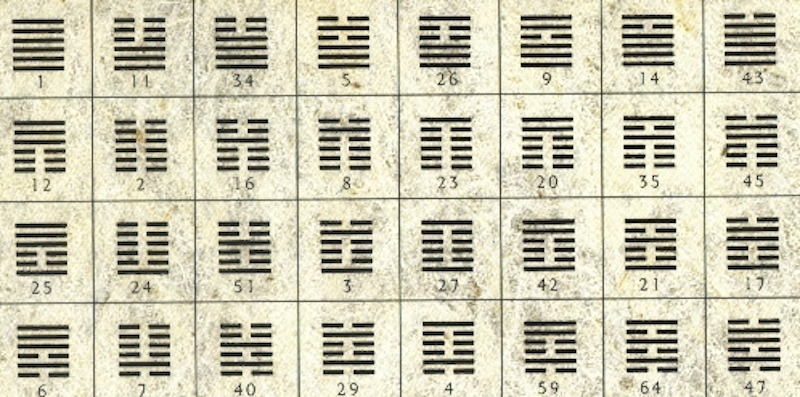
\includegraphics[width=\paperwidth,height=\paperheight]{i-ching.jpg}}
  \end{frame}
  \begin{frame}[c]
  	\centering
  	\Huge
  	The Man in the High Castle
  	
  	1962
  \end{frame}

\begin{frame}[plain]
	\makebox[\linewidth]{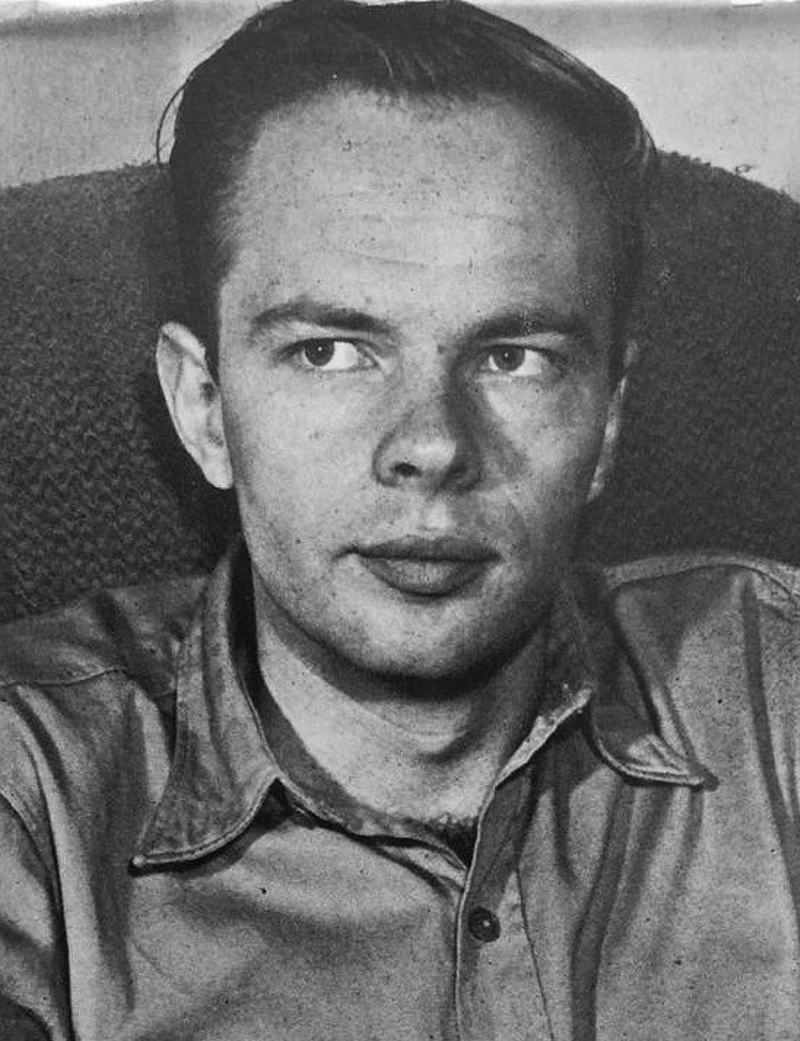
\includegraphics[height=\paperheight]{pkd.jpg}}
\end{frame}

\begin{frame}[c]
	\centering
	\Huge
	Bibliomancy
	
	(1753 - as a term)
\end{frame}

\begin{frame}[plain]
	\makebox[\linewidth]{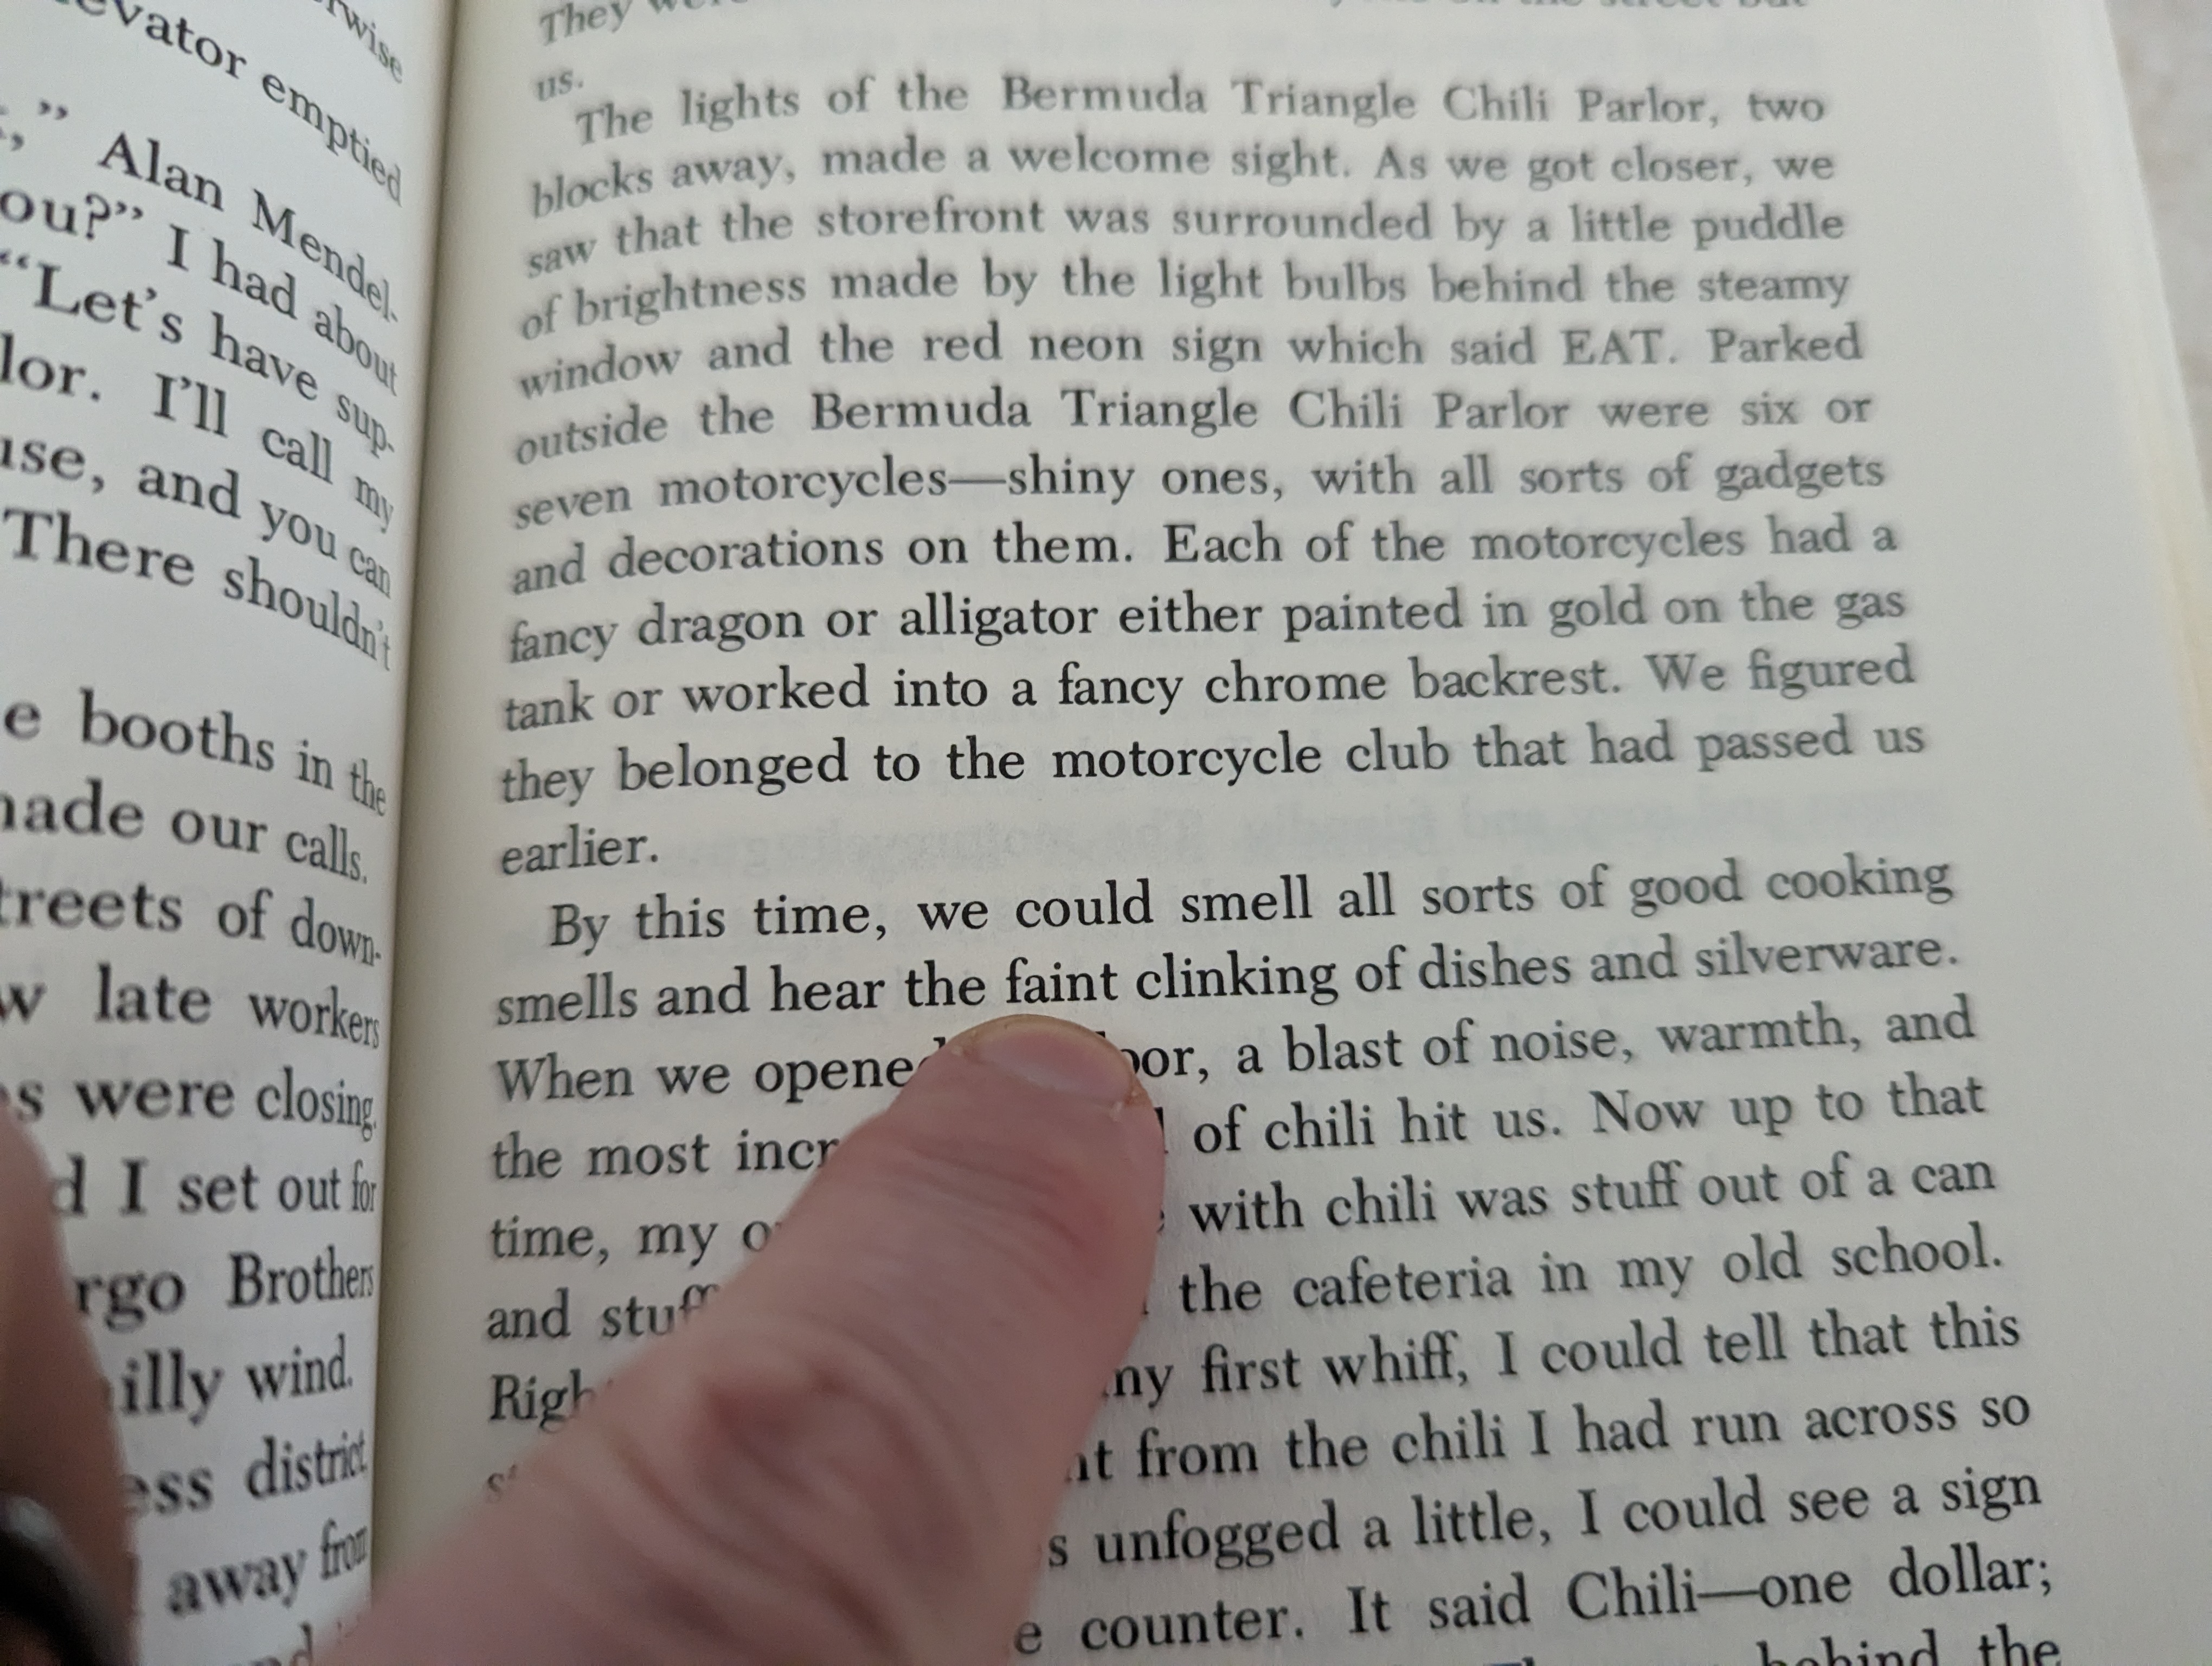
\includegraphics[width=\paperwidth,height=\paperheight]{pinkwater-bibliomancy.jpg}}
\end{frame}

\begin{frame}[c]
	\centering
	\Huge
	The Cut-Up Technique
	
	(1920s)
\end{frame}

\begin{frame}[plain]
	\makebox[\linewidth]{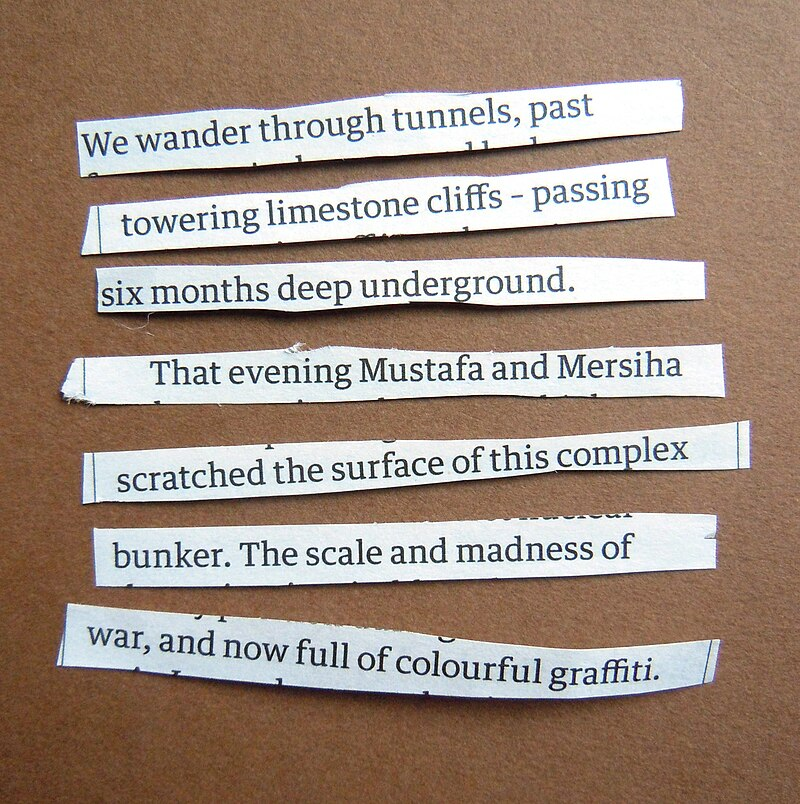
\includegraphics[width=\paperwidth,height=\paperheight]{cut-up.jpg}}
\end{frame}

%The 1958 / Danny Dunn thing should probably go right before you actually talk about LLMs

\begin{frame}[c]
	\centering
	\Huge
	1958
\end{frame}

\begin{frame}[plain]
	\makebox[\linewidth]{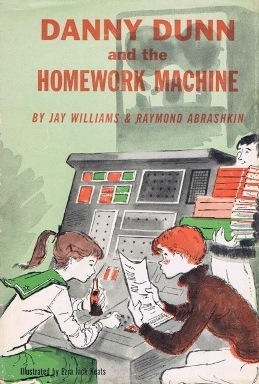
\includegraphics[height=\paperheight]{dannydunn.jpg}}
\end{frame}

\end{document}
